\documentclass[11pt,a4paper]{article}
 
\newcommand{\tumsoTime}{13:00 น. - 16:00 น.}
\newcommand{\tumsoRound}{2}
 
\usepackage{../tumso}
 \usepackage{tikz}
 
\begin{document}
 
\begin{problem}{สามเหลี่ยม}{}{}{0.25 second}{32 megabytes}{100}

มีจุดอยู่ $N$ จุดบนแกนพิกัด $2$ มิติ ให้หาพื้นที่ของสามเหลี่ยมที่มากที่สุดที่เกิดจาก $3$ จุดใดๆ ใน $N$ จุดนี้


เช่น $N = 7$ มีจุดดังรูป

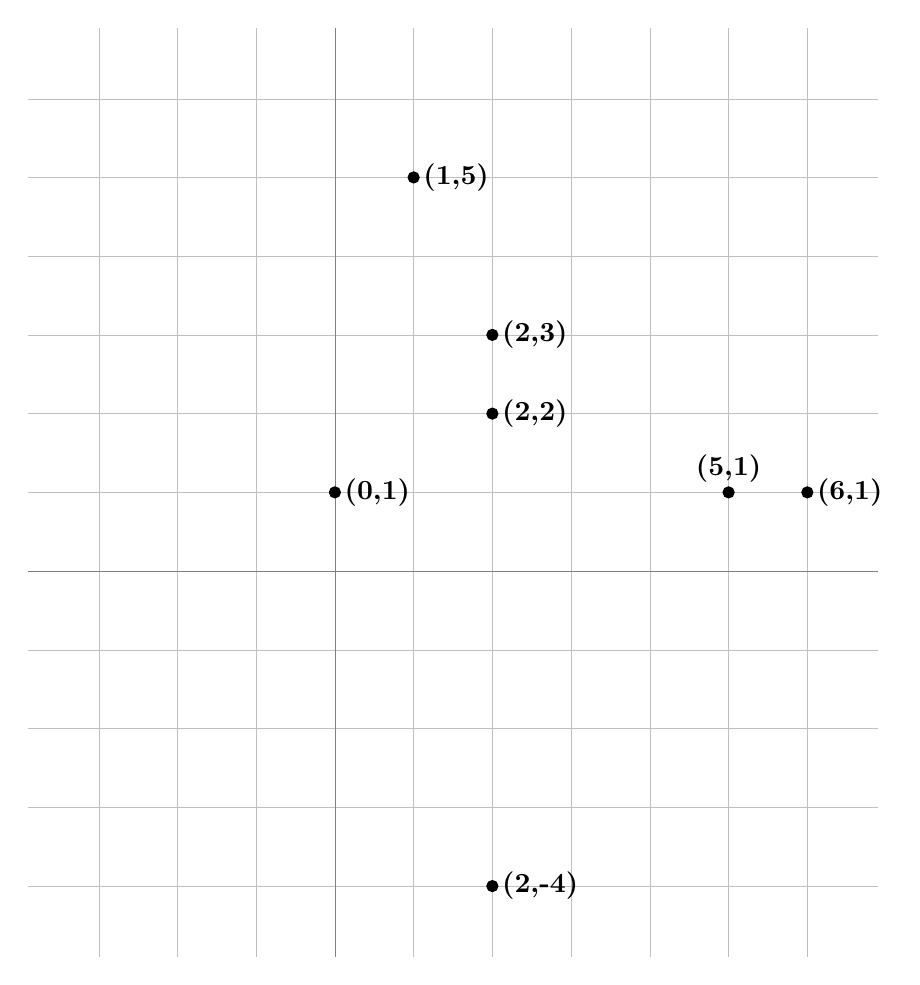
\begin{tikzpicture}
\draw[step=1cm,lightgray,ultra thin] (-3.9,-4.9) grid (6.9,6.9);
\draw[gray, ultra thin] (0,-4.9) -- (0,6.9);
\draw[gray, ultra thin] (-3.9,0) -- (6.9,0);
\filldraw[black] (1,5) circle (2pt) node[anchor=west]{\textbf{(1,5)}};
\filldraw[black] (2,3) circle (2pt) node[anchor=west]{\textbf{(2,3)}};
\filldraw[black] (2,-4) circle (2pt) node[anchor=west]{\textbf{(2,-4)}};
\filldraw[black] (6,1) circle (2pt) node[anchor=west]{\textbf{(6,1)}};
\filldraw[black] (2,2) circle (2pt) node[anchor=west]{\textbf{(2,2)}};
\filldraw[black] (0,1) circle (2pt) node[anchor=west]{\textbf{(0,1)}};
\filldraw[black] (5,1) circle (2pt) node[anchor=south]{\textbf{(5,1)}};
\end{tikzpicture}

เห็นได้ว่าสามเหลี่ยมที่มีพื้นที่มากที่สุดคือสามเหลี่ยมสีแดงดังรูป

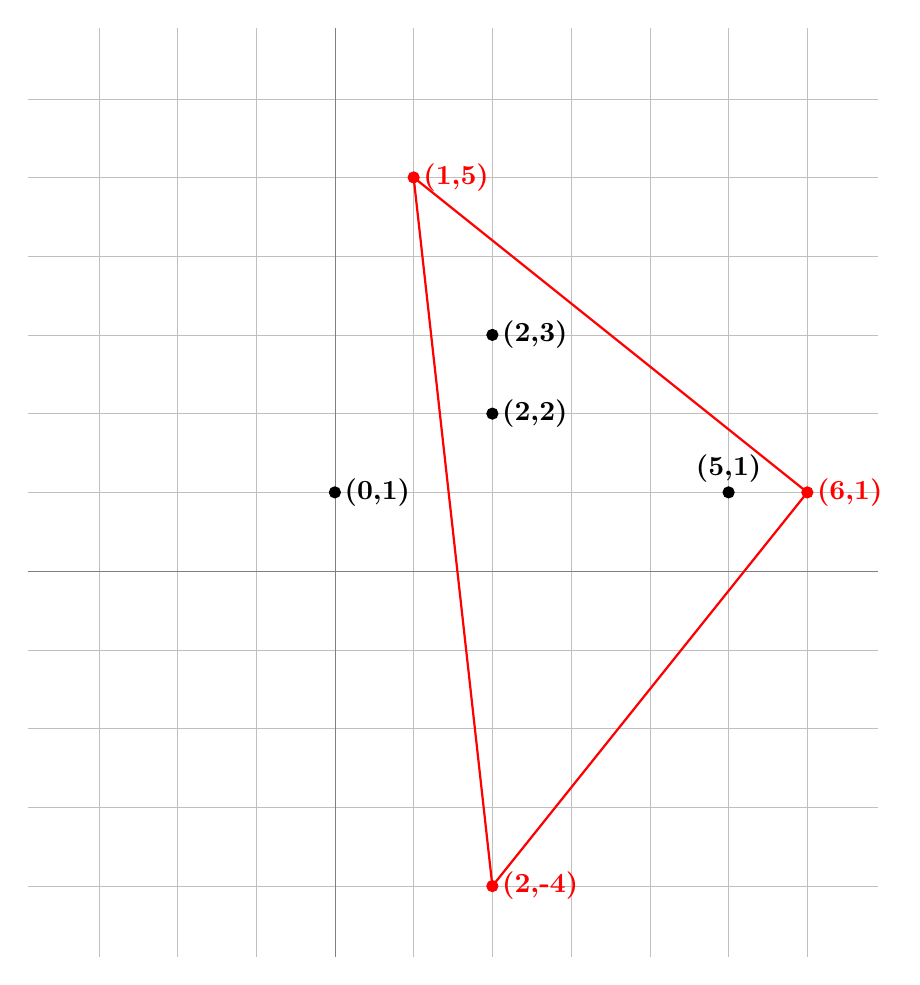
\begin{tikzpicture}
\draw[step=1cm,lightgray,ultra thin] (-3.9,-4.9) grid (6.9,6.9);
\draw[gray, ultra thin] (0,-4.9) -- (0,6.9);
\draw[gray, ultra thin] (-3.9,0) -- (6.9,0);
\draw[red, thick] (1,5) -- (2,-4);
\draw[red, thick] (1,5) -- (6,1);
\draw[red, thick] (2,-4) -- (6,1);

\filldraw[red] (1,5) circle (2pt) node[anchor=west]{\textbf{(1,5)}};
\filldraw[black] (2,3) circle (2pt) node[anchor=west]{\textbf{(2,3)}};
\filldraw[red] (2,-4) circle (2pt) node[anchor=west]{\textbf{(2,-4)}};
\filldraw[red] (6,1) circle (2pt) node[anchor=west]{\textbf{(6,1)}};
\filldraw[black] (2,2) circle (2pt) node[anchor=west]{\textbf{(2,2)}};
\filldraw[black] (0,1) circle (2pt) node[anchor=west]{\textbf{(0,1)}};
\filldraw[black] (5,1) circle (2pt) node[anchor=south]{\textbf{(5,1)}};
\end{tikzpicture}

พื้นที่สามเหลี่ยมรูปนี้คือ 20.5 ตารางหน่วย ดังนั้นต้องตอบว่า 20.500

\InputFile

บรรทัดแรก ระบุจำนวนเต็ม $N$ $(3 \leq N \leq 10^5)$ โดยที่ $N$ แทนจำนวนจุด

บรรทัดที่ $1+i$ $(1 \leq i \leq N)$ แต่ละบรรทัดระบุจำนวนเต็ม $2$ ตัว ระบุ $X_i, Y_i$ $(-10^8 \leq X_i, Y_i \leq 10^8)$ ตามลำดับโดยที่ $(X_i,Y_i)$ แทนพิกัดจุดที่ $i$

\OutputFile

$1$ บรรทัด แสดงพื้นที่ของสามเหลี่ยมที่ใหญ่ที่สุดที่เกิดจากจุด $N$ จุดนี้ ให้ตอบเป็นทศนิยม 3 ตำแหน่ง

\Scoring
ชุดทดสอบจะถูกแบ่งเป็น 3 ชุด จะได้คะแนนในแต่ละชุดก็ต่อเมื่อโปรแกรมให้ผลลัพธ์ถูกต้องในชุดทดสอบย่อยทั้งหมด
 
\begin{description}
\item[ชุดที่ 1 (7 คะแนน)] $N \leq 20$
\item[ชุดที่ 2 (30 คะแนน)] $N \leq 2000$
\item[ชุดที่ 3 (63 คะแนน)] ไม่มีเงื่อนไขเพิ่มเติม
\end{description}

\Examples

\begin{example}
\exmp{7
1 5
2 3
2 2
0 1
2 -4
5 1
6 1
}{20.500
}%
\end{example}
 
\end{problem}
 
\end{document}